En este apartado se detallan los resultados obtenidos en la realización de las pruebas de accesibilidad del sistema.
Se han realizado pruebas de accesibilidad en las distintas vistas de la aplicación, comprobando que se cumplen los requisitos de accesibilidad definidos en la sección \hyperlink{sec:6_2-RNF}{\ref*{sec:6_2-RNF} \nameref*{sec:6_2-RNF}}.

Se muestran a continuación los resultados obtenidos en las pruebas de accesibilidad realizadas en las vistas principales de la aplicación.
Estos resultados han sido obtenidos de la herramienta de evaluación de accesibilidad \textit{WAVE}.

\subsection*{Home}
\begin{itemize}
    \item \textbf{Resultado:} La vista principal de la aplicación cumple con los requisitos de accesibilidad.
    \item \textbf{Observaciones:} Los errores de contraste se deben a los colores de las cartas de ejemplo y son aceptados.
\end{itemize}

\begin{figure}[H]
    \centering
    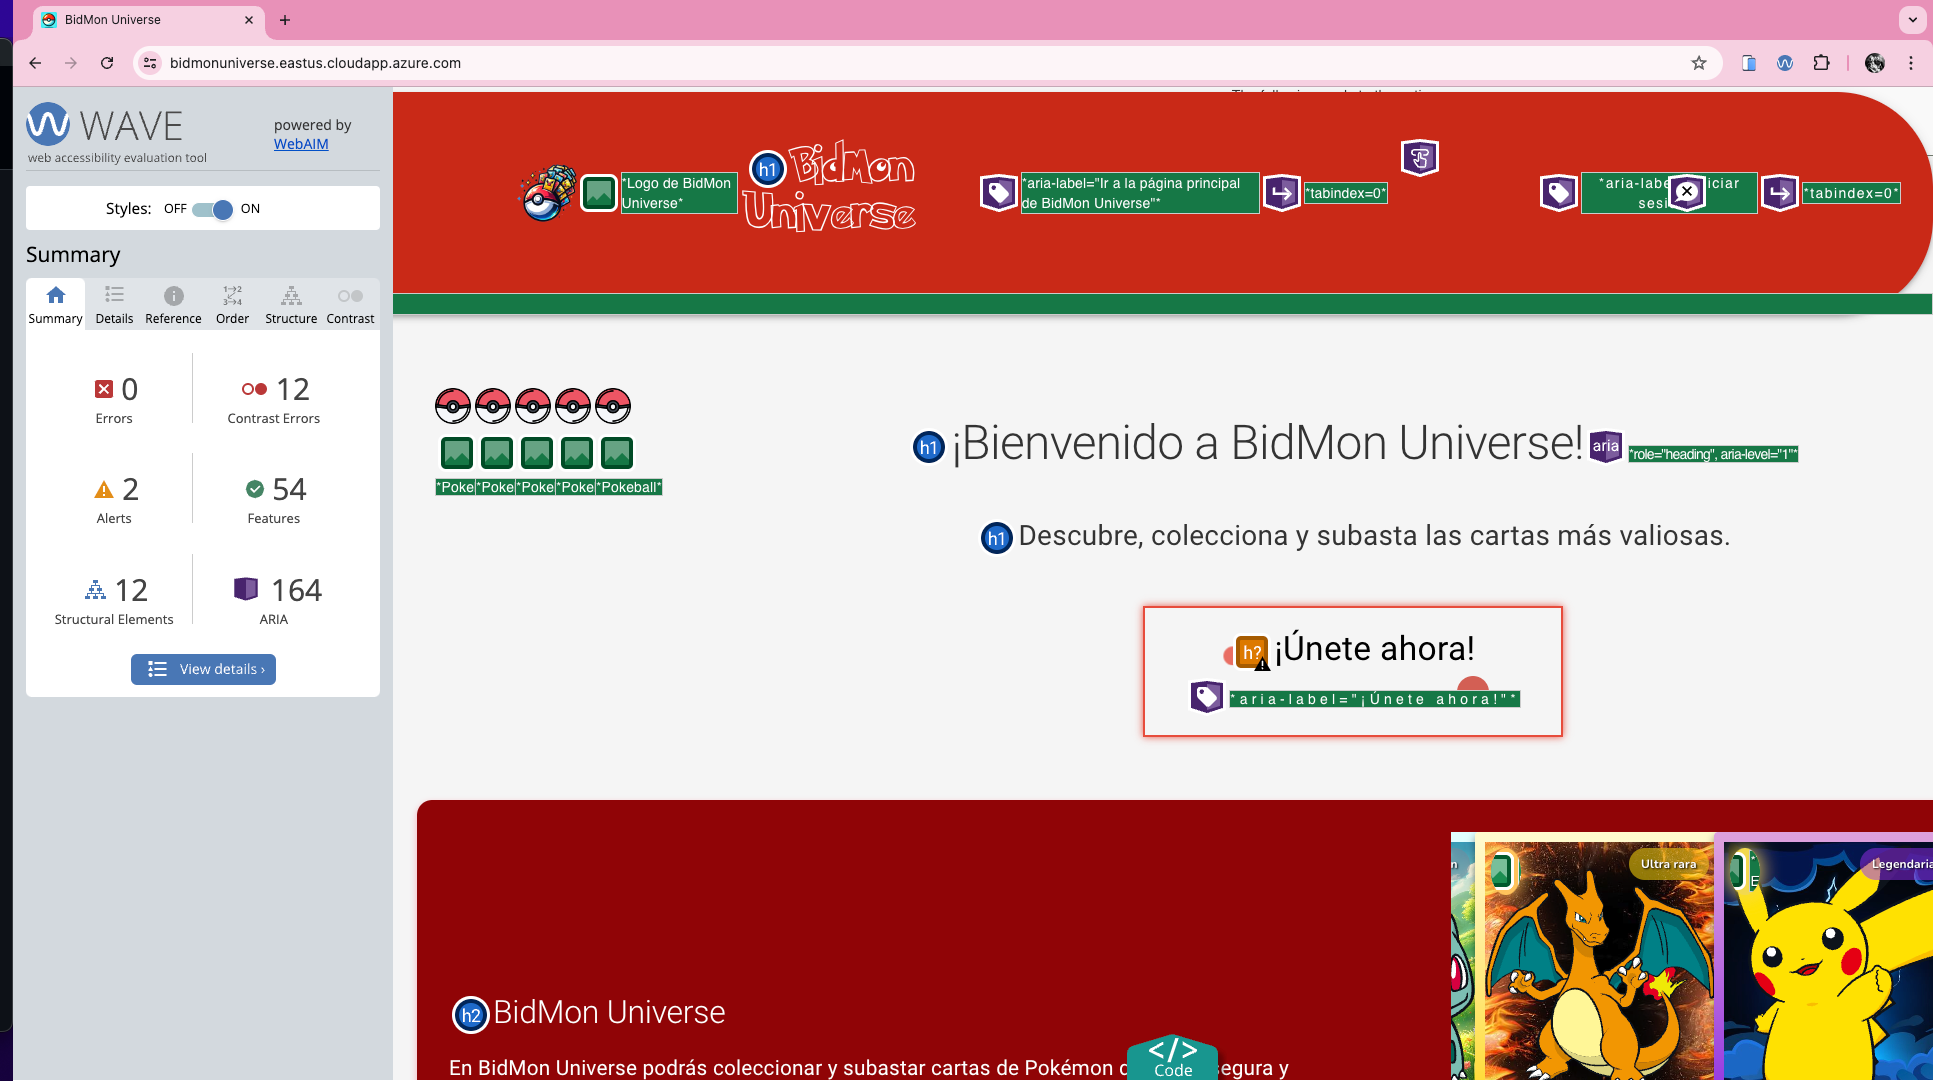
\includegraphics[width=0.8\textwidth]{figures/accesibilidad/A-acc-home.png}
    \caption{Accesibilidad Página Home}
    \label{fig:Acc-Home}
\end{figure}

\subsection*{Acerca de}
\begin{itemize}
    \item \textbf{Resultado:} La vista de información sobre la aplicación cumple con los requisitos de accesibilidad.
\end{itemize}

\begin{figure}[H]
    \centering
    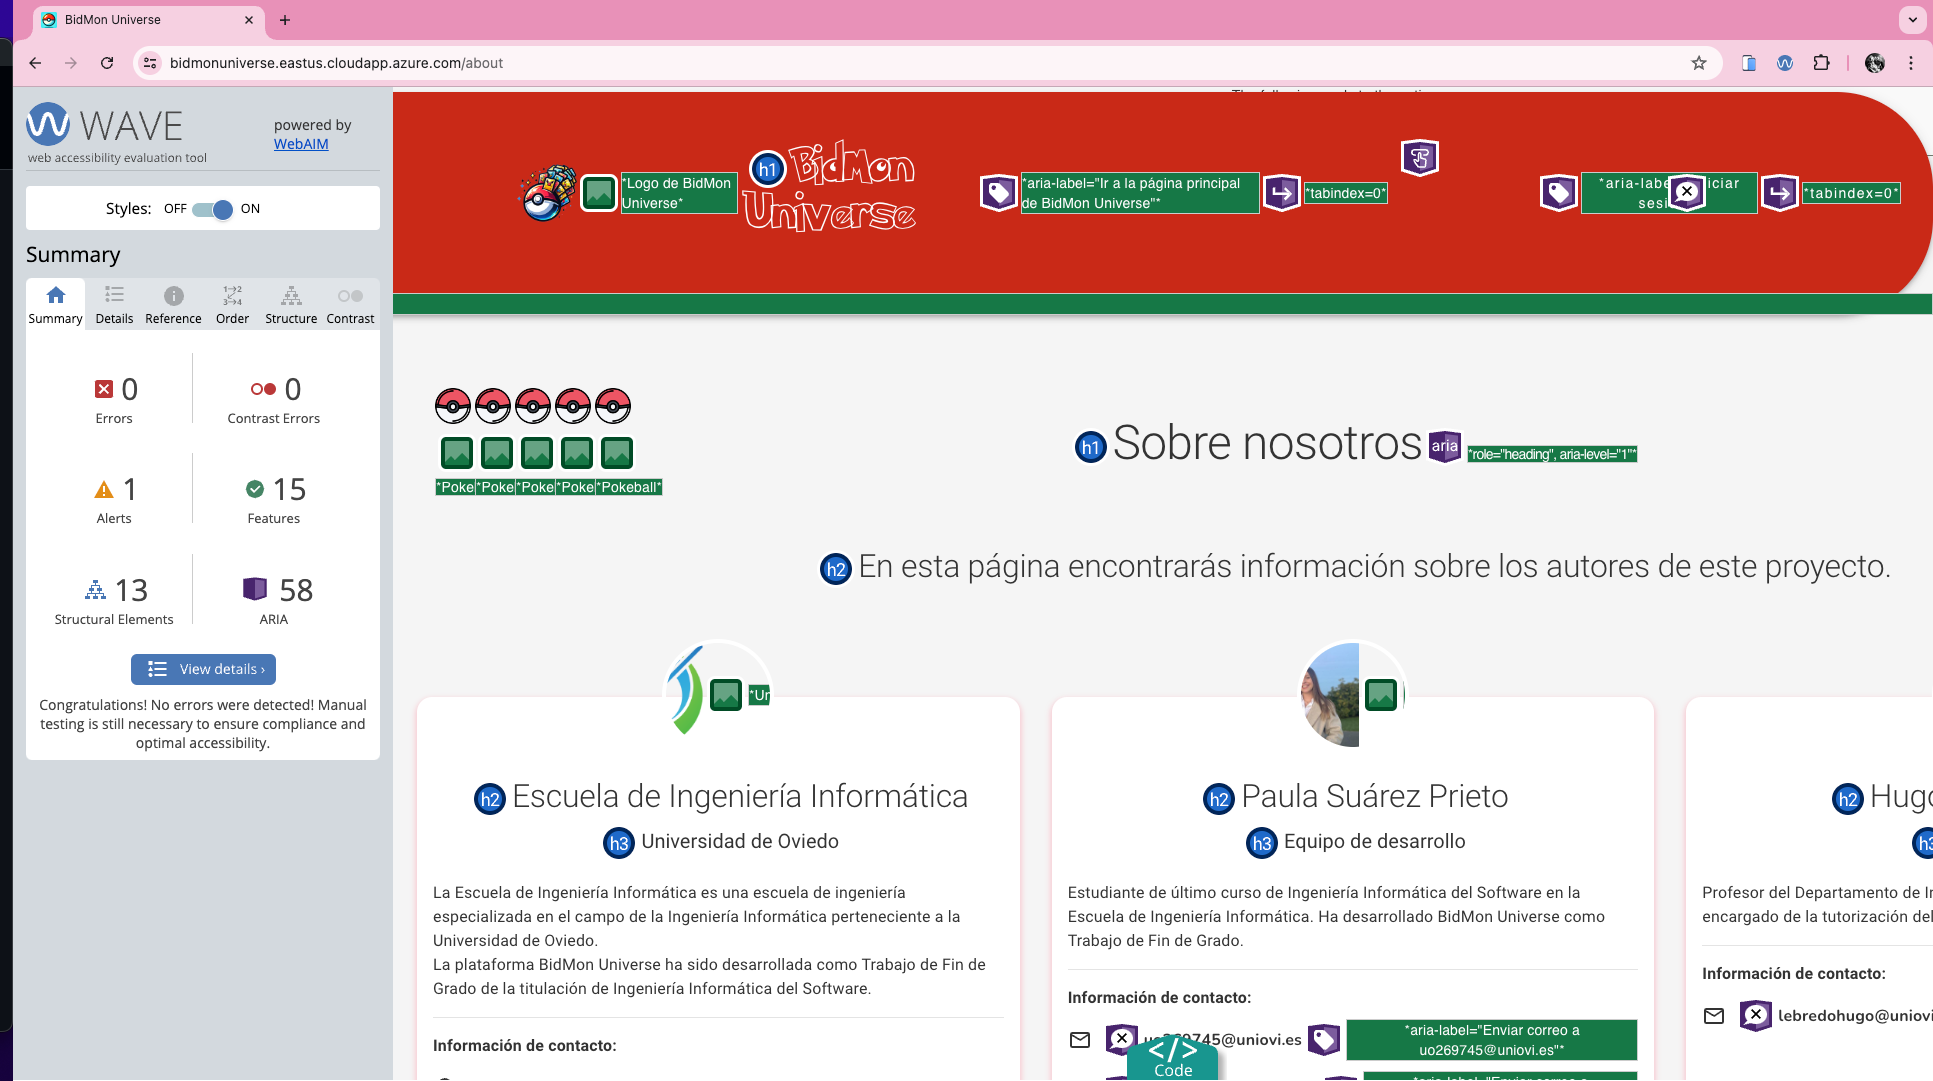
\includegraphics[width=0.8\textwidth]{figures/accesibilidad/A-acc-about.png}
    \caption{Accesibilidad Página Acerca de}
    \label{fig:Acc-Acerca}
\end{figure}

\subsection*{Login}
\begin{itemize}
    \item \textbf{Resultado:} La vista de inicio de sesión cumple con los requisitos de accesibilidad.
\end{itemize}

\begin{figure}[H]
    \centering
    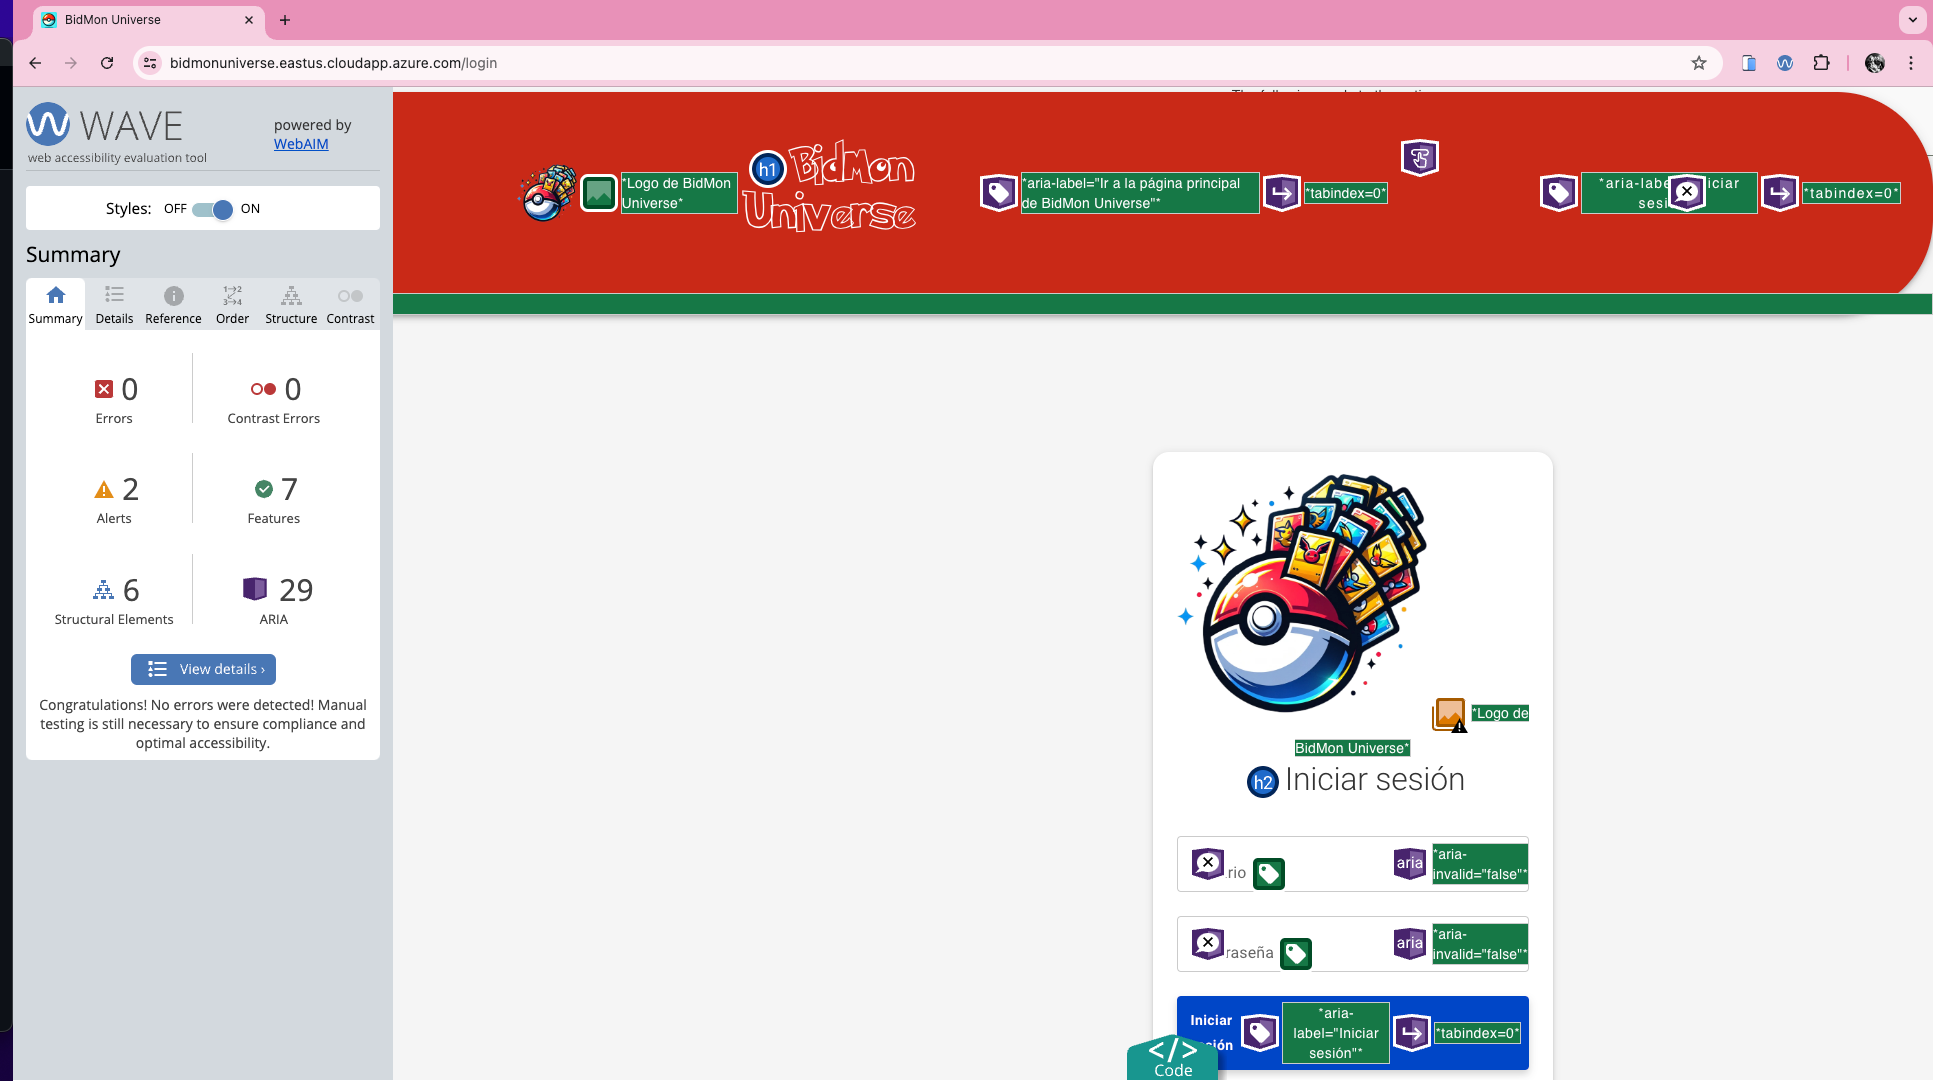
\includegraphics[width=0.8\textwidth]{figures/accesibilidad/A-acc-login.png}
    \caption{Accesibilidad Página Login}
    \label{fig:Acc-Login}
\end{figure}

\subsection*{Registro}
\begin{itemize}
    \item \textbf{Resultado:} La vista de registro cumple con los requisitos de accesibilidad.
\end{itemize}

\begin{figure}[H]
    \centering
    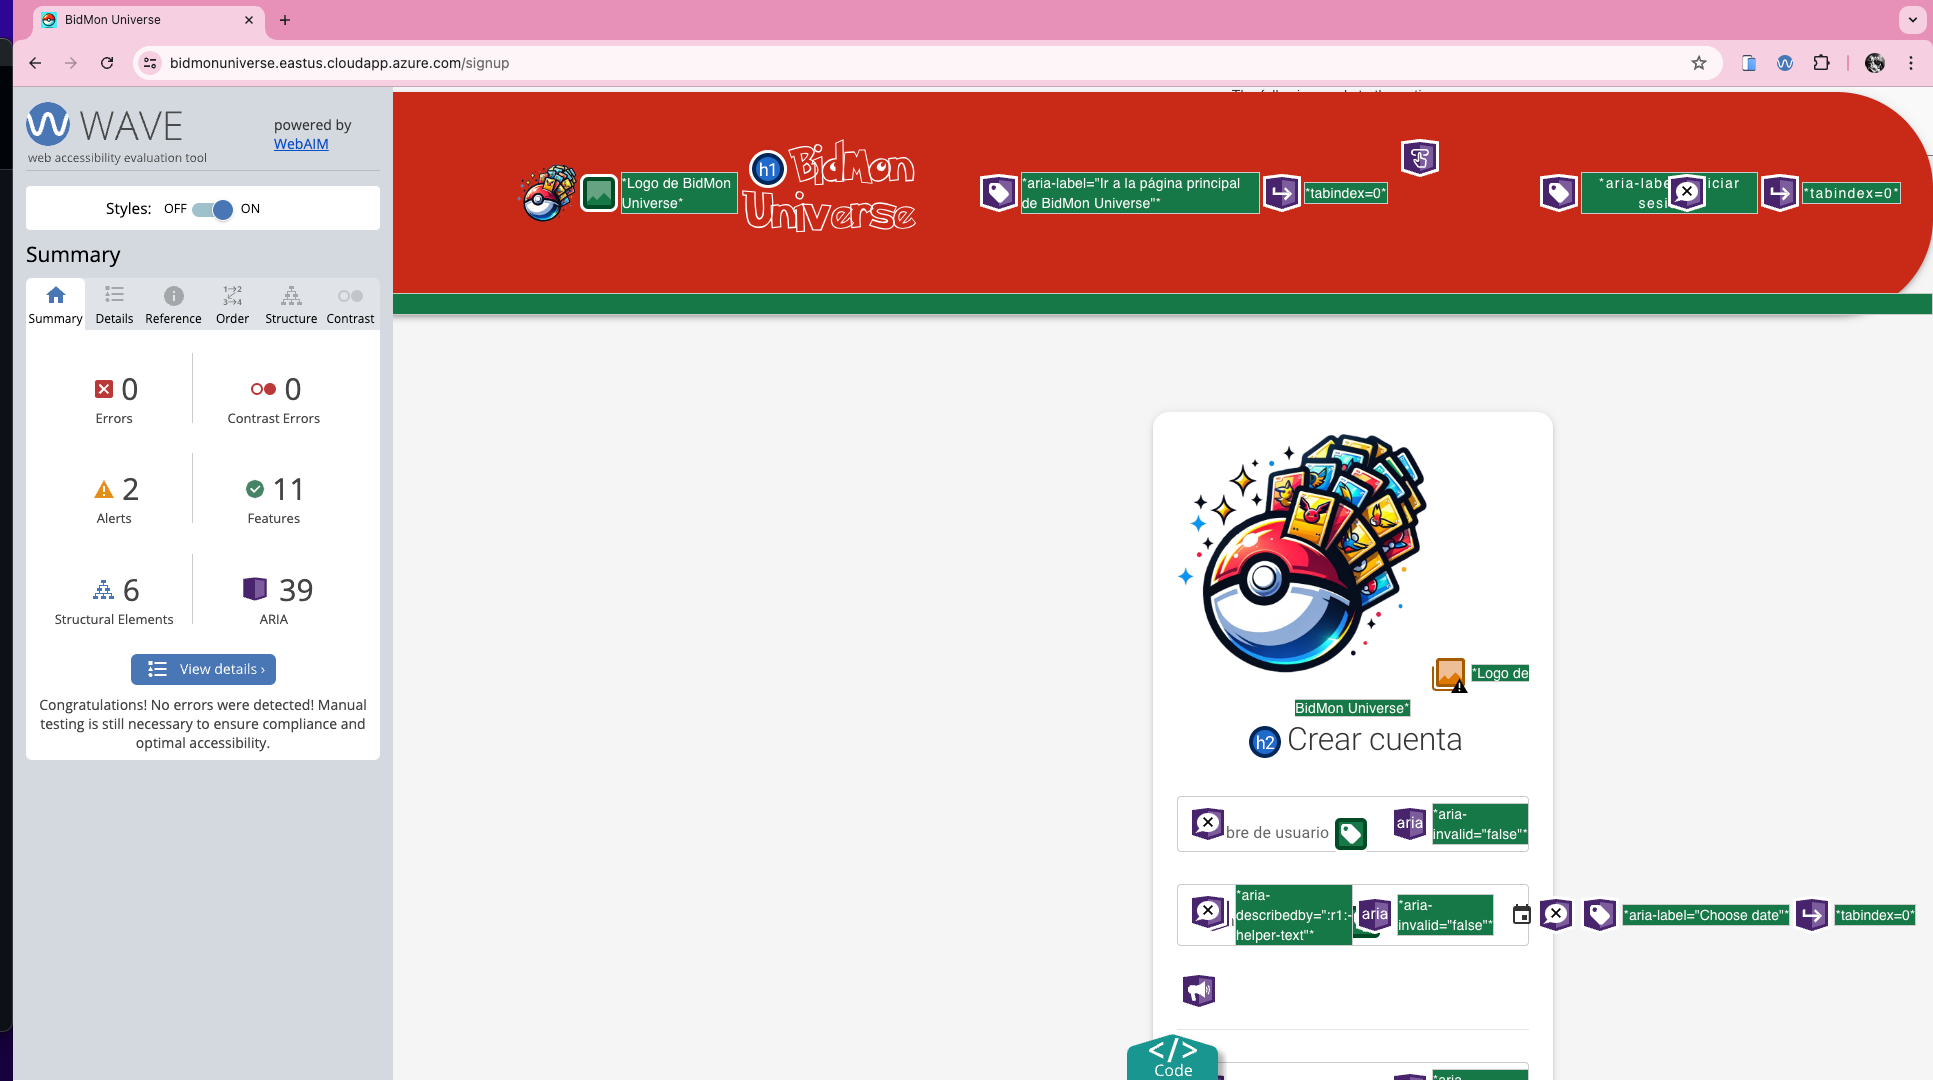
\includegraphics[width=0.8\textwidth]{figures/accesibilidad/A-acc-registro.png}
    \caption{Accesibilidad Página Registro}
    \label{fig:Acc-Registro}
\end{figure}


\subsection*{Perfil}
\begin{itemize}
    \item \textbf{Resultado:} La vista de perfil cumple con los requisitos de accesibilidad.
\end{itemize}

\begin{figure}[H]
    \centering
    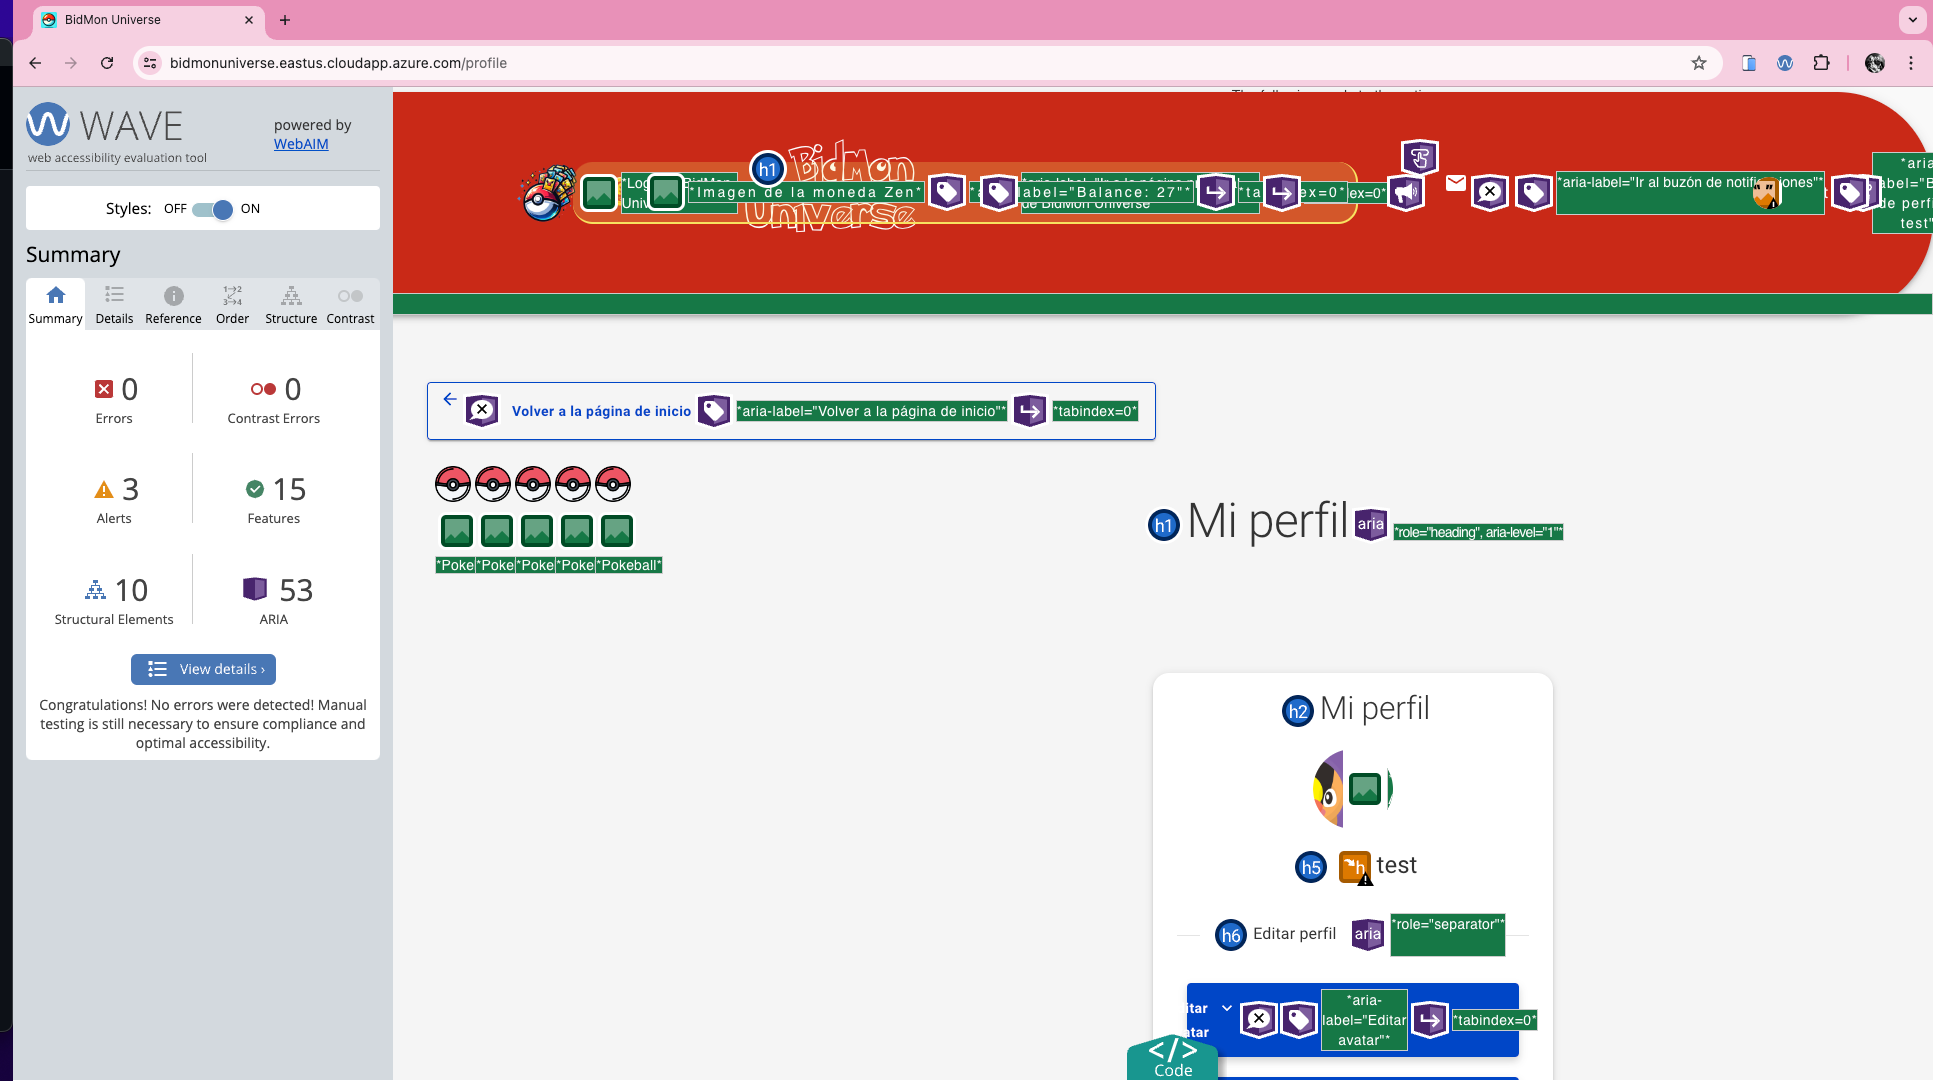
\includegraphics[width=0.8\textwidth]{figures/accesibilidad/A-acc-perfil.png}
    \caption{Accesibilidad Página Perfil}
    \label{fig:Acc-Perfil}
\end{figure}


\subsection*{Página principal de usuario autenticado}
\begin{itemize}
    \item \textbf{Resultado:} La vista principal de usuario autenticado cumple con los requisitos de accesibilidad.
    \item \textbf{Observaciones:} Los errores de contraste se deben a los colores de las cartas y son aceptados.
\end{itemize}


\begin{figure}[H]
    \centering
    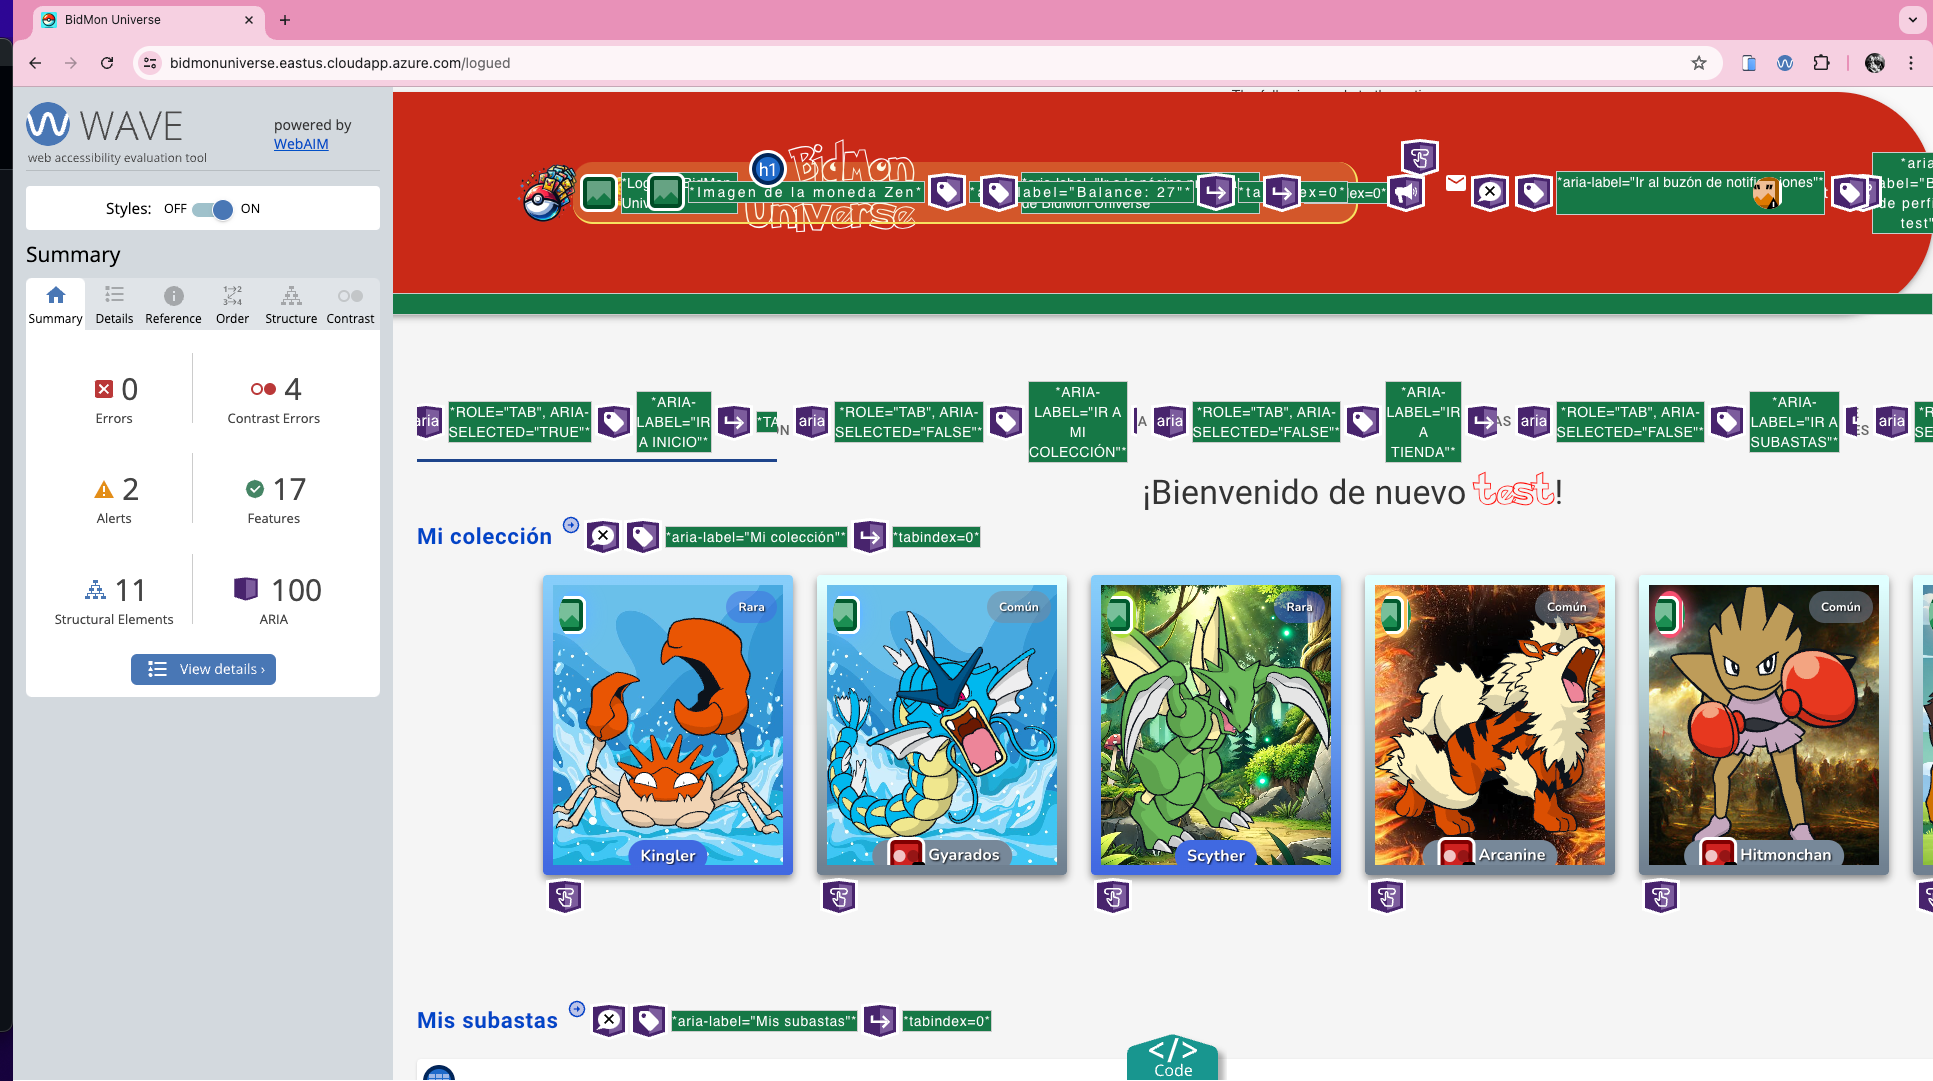
\includegraphics[width=0.8\textwidth]{figures/accesibilidad/A-acc-logued.png}
    \caption{Accesibilidad Página principal de usuario autenticado}
    \label{fig:Acc-Principal-Usuario}
\end{figure}

\subsection*{Colección de cartas del usuario}
\begin{itemize}
    \item \textbf{Resultado:} La vista de colección de cartas del usuario cumple con los requisitos de accesibilidad.
    \item \textbf{Observaciones:} Los errores de contraste se deben a los colores de las cartas y son aceptados.
\end{itemize}

\begin{figure}[H]
    \centering
    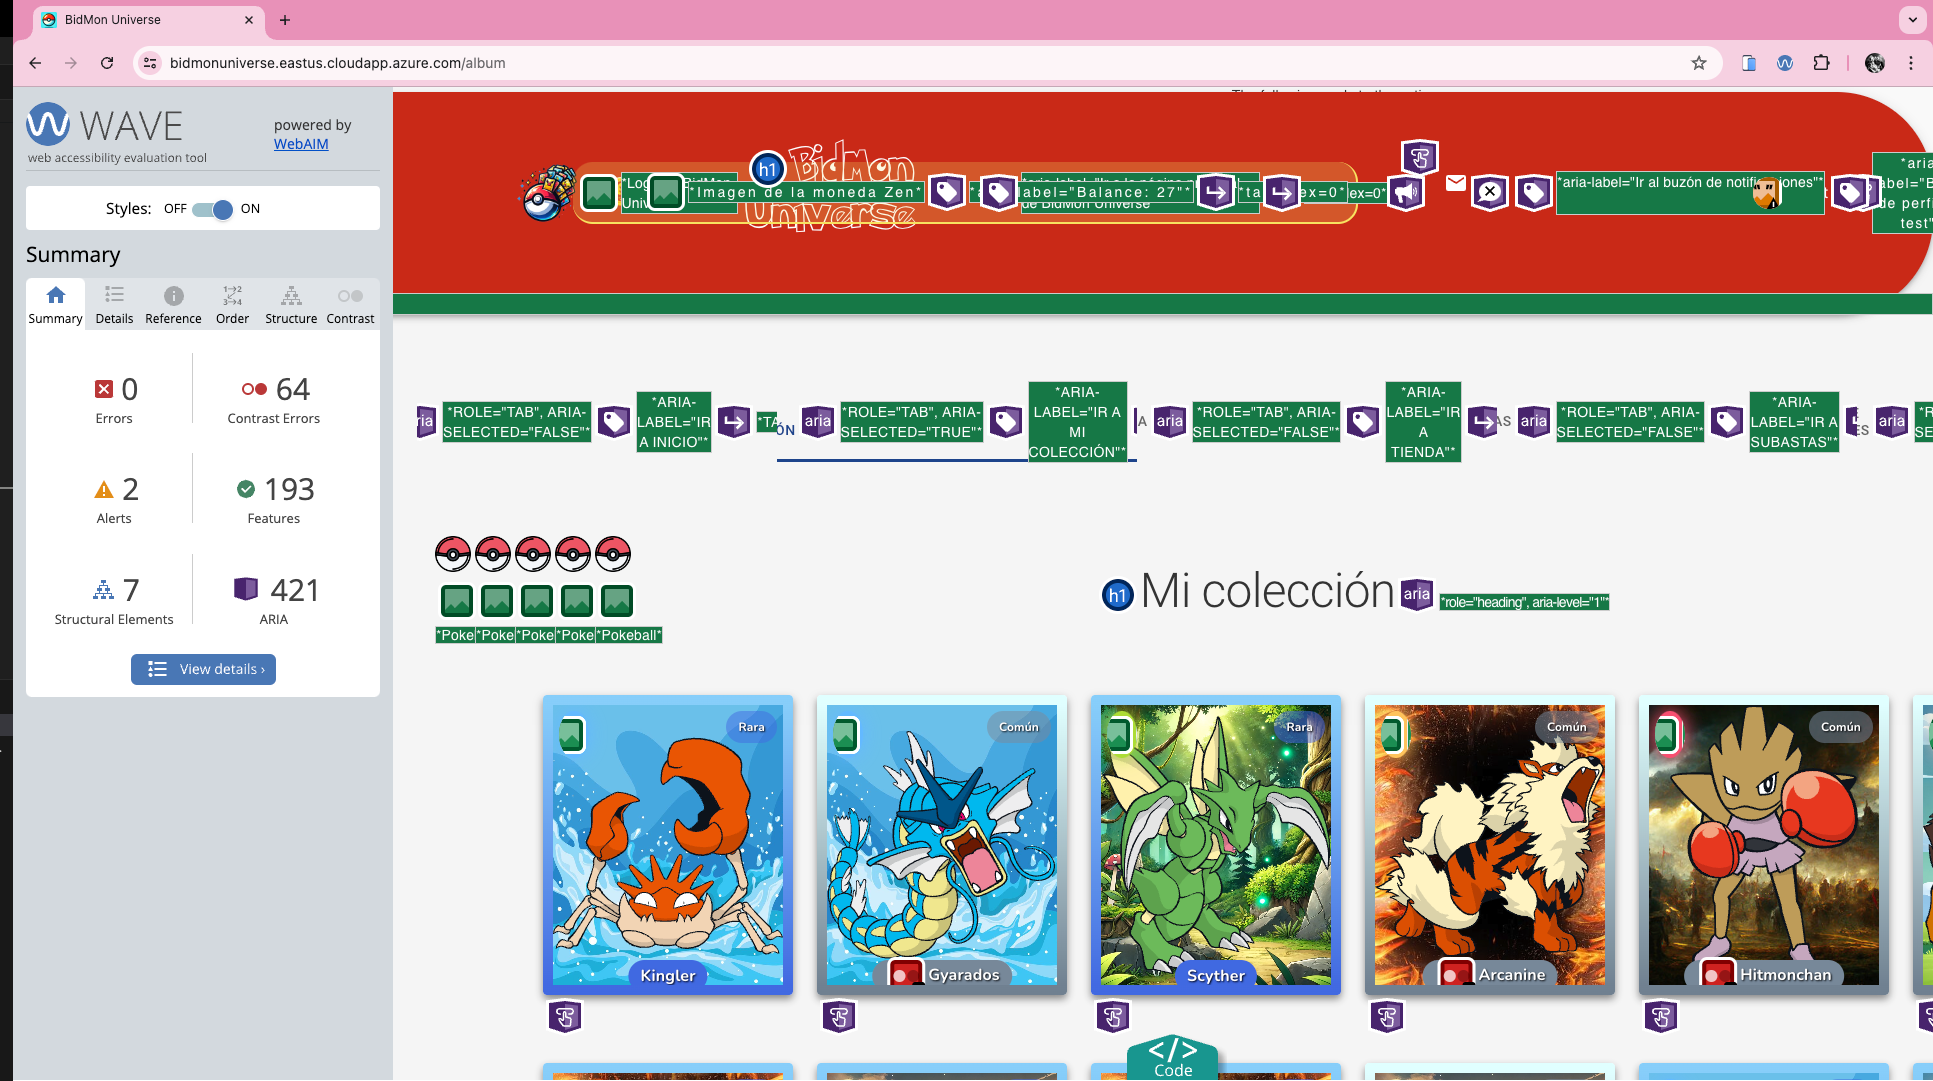
\includegraphics[width=0.8\textwidth]{figures/accesibilidad/A-acc-coleccion.png}
    \caption{Accesibilidad Página Colección de cartas del usuario}
    \label{fig:Acc-Coleccion}
\end{figure}


\subsection*{Tienda}
\begin{itemize}
    \item \textbf{Resultado:} La vista de la tienda cumple con los requisitos de accesibilidad.
\end{itemize}

\begin{figure}[H]
    \centering
    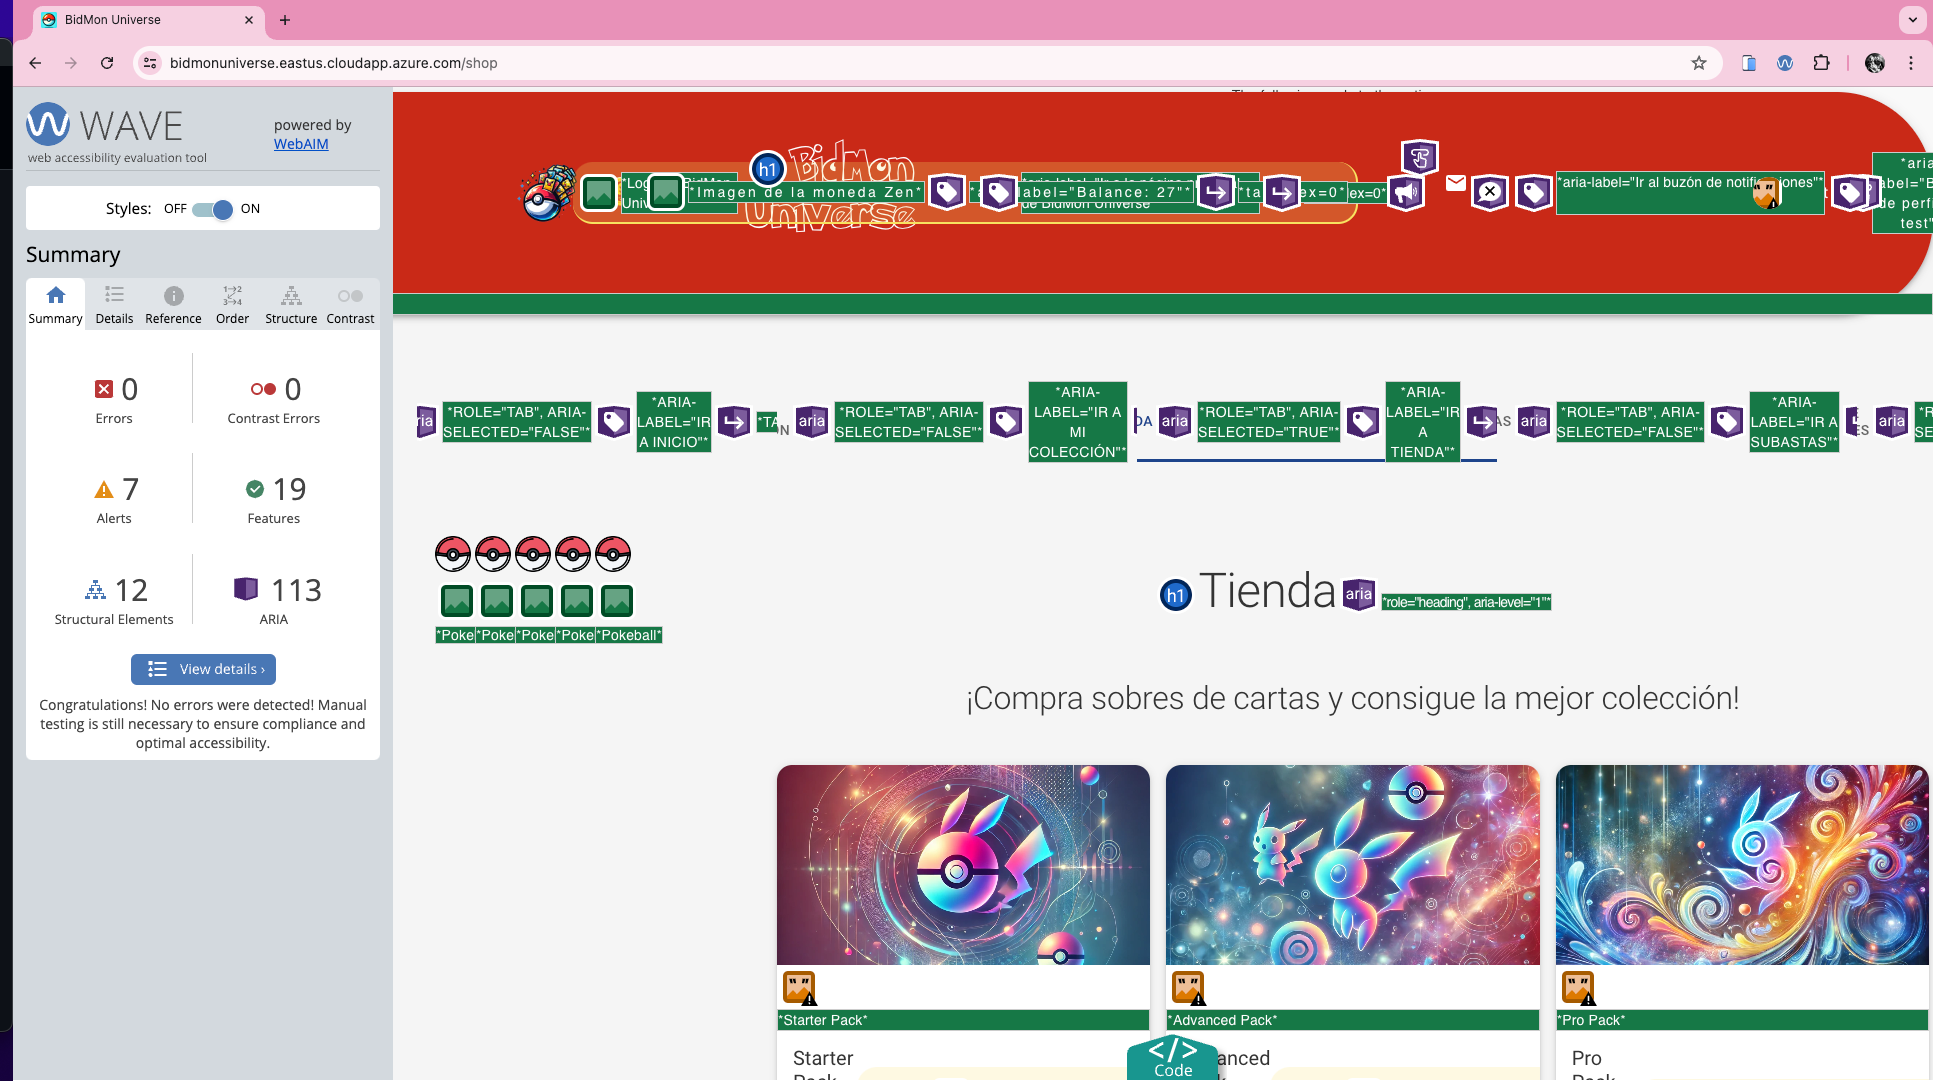
\includegraphics[width=0.8\textwidth]{figures/accesibilidad/A-acc-tienda.png}
    \caption{Accesibilidad Página Tienda}
    \label{fig:Acc-Tienda}
\end{figure}

\subsection*{Recarga de saldo}
\begin{itemize}
    \item \textbf{Resultado:} La vista de recarga de saldo cumple con los requisitos de accesibilidad.
\end{itemize}

\begin{figure}[H]
    \centering
    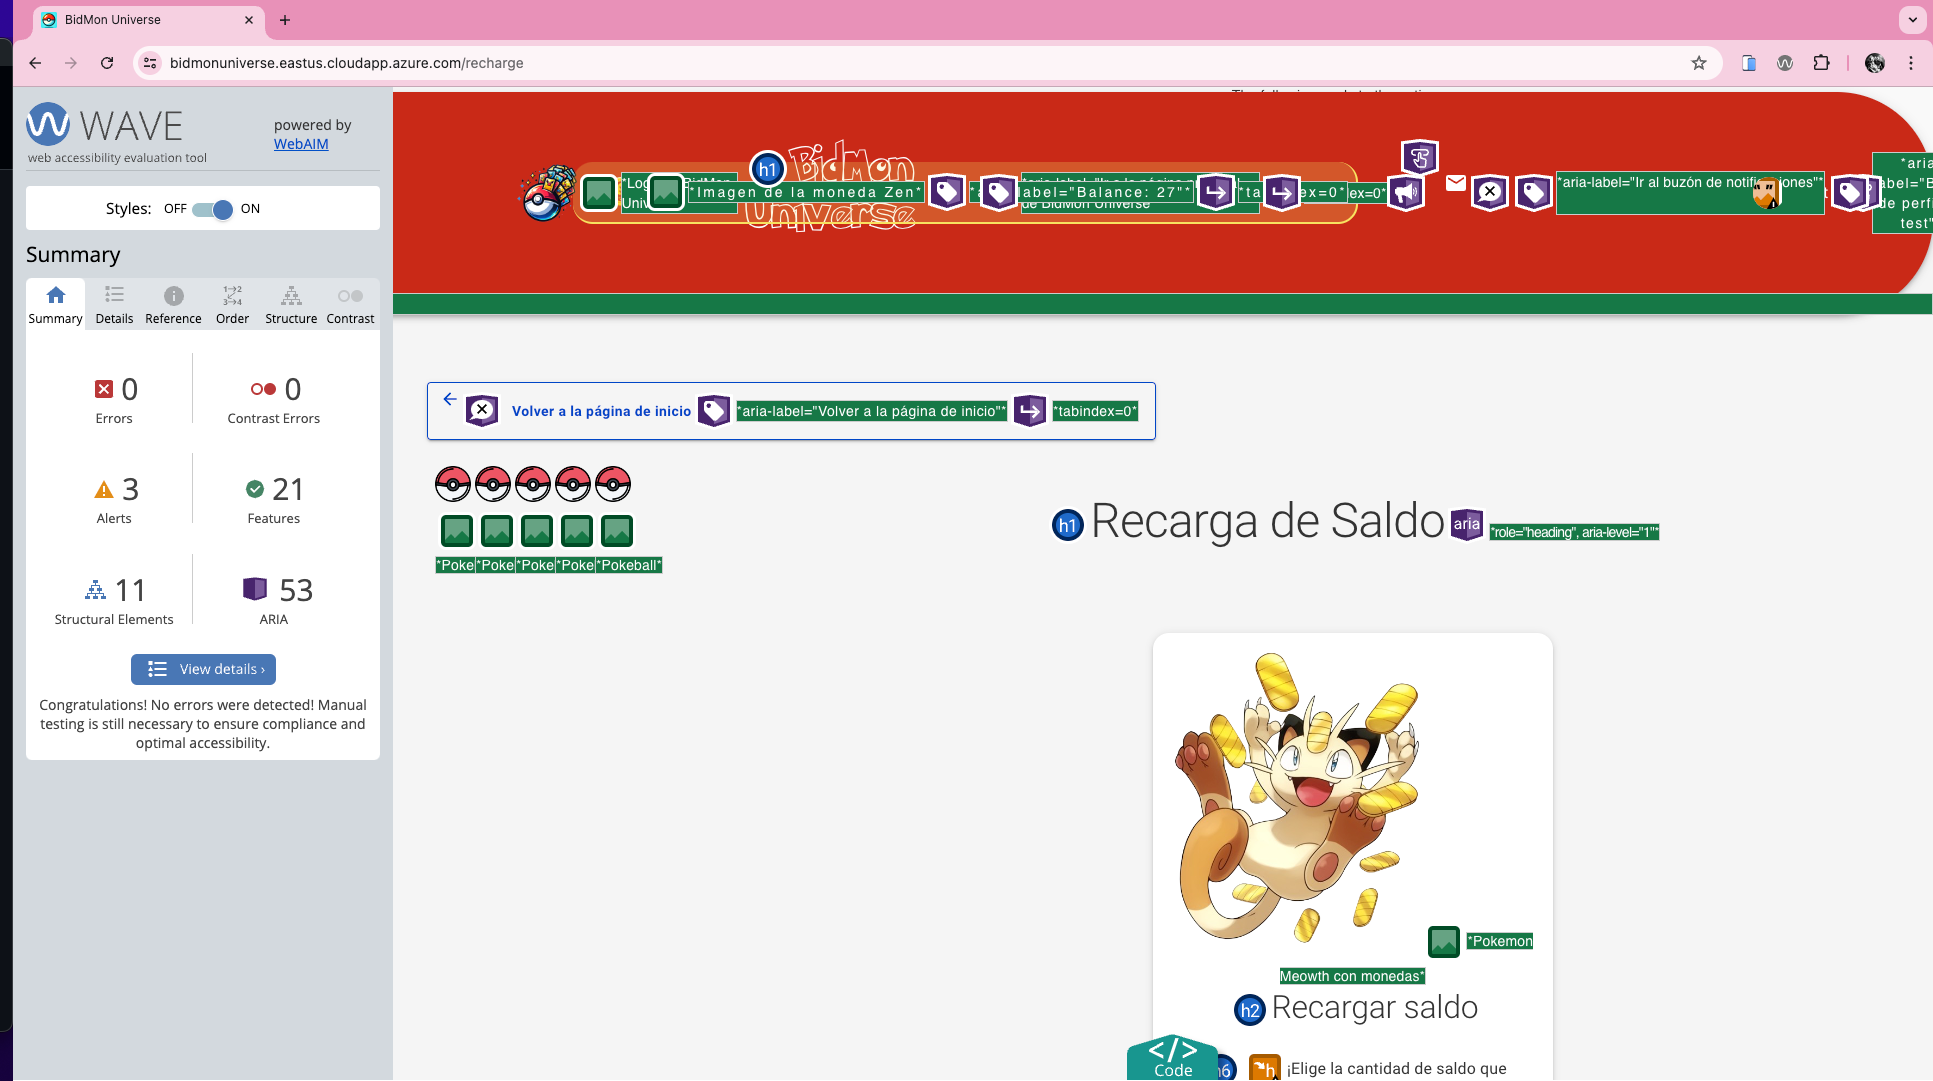
\includegraphics[width=0.8\textwidth]{figures/accesibilidad/A-acc-recarga.png}
    \caption{Accesibilidad Página Recarga de saldo}
    \label{fig:Acc-Recarga}
\end{figure}

\subsection*{Subastas activas}
\begin{itemize}
    \item \textbf{Resultado:} La vista de subastas activas cumple con los requisitos de accesibilidad.
    \item \textbf{Observaciones:} Los errores de contraste se deben a los colores de las cartas y son aceptados.
\end{itemize}

\begin{figure}[H]
    \centering
    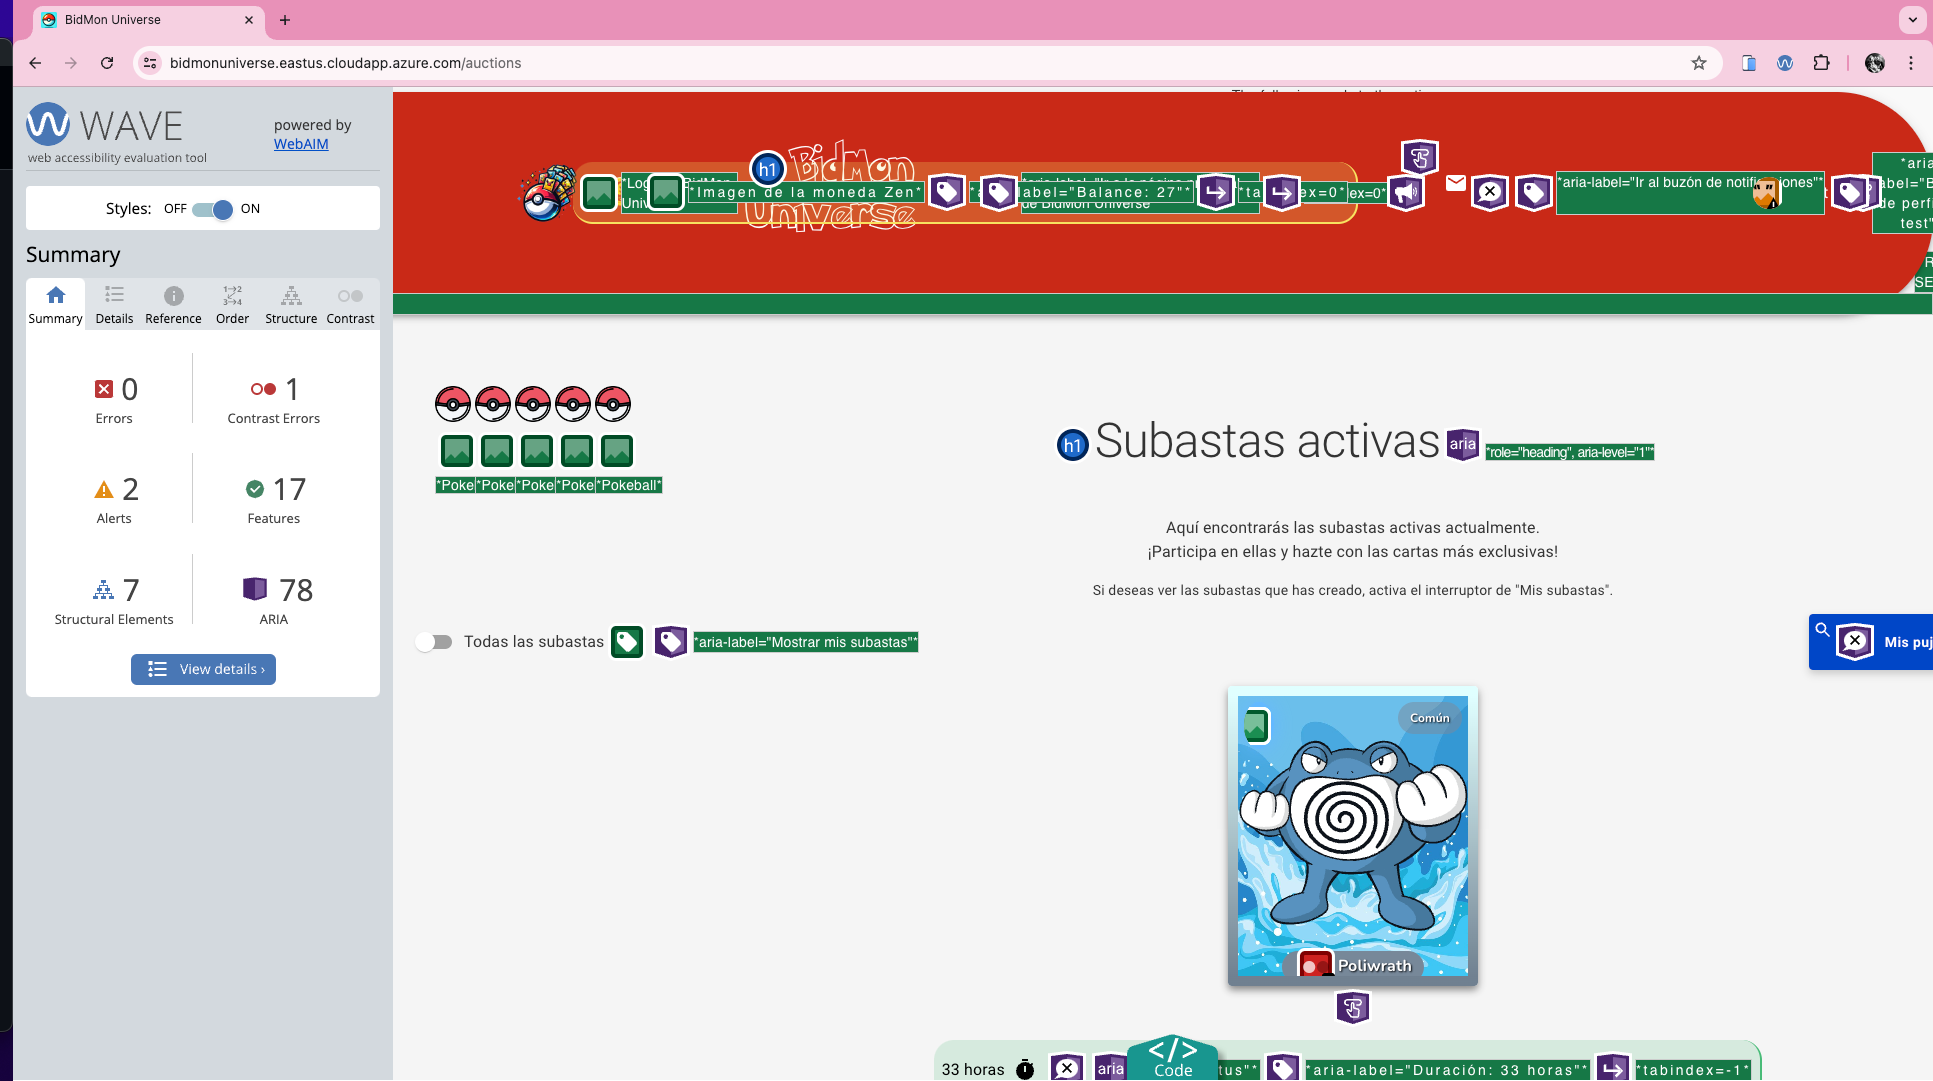
\includegraphics[width=0.8\textwidth]{figures/accesibilidad/A-acc-subastas.png}
    \caption{Accesibilidad Página Subastas activas}
    \label{fig:Acc-Subastas}
\end{figure}

\subsection*{Detalle de una carta}
\begin{itemize}
    \item \textbf{Resultado:} La vista de detalle de una carta cumple con los requisitos de accesibilidad.
    \item \textbf{Observaciones:} Dependiendo de la carta que se consulte se puede obtener un error de contraste se debe al color de la carta y es aceptado.
\end{itemize}

\begin{figure}[H]
    \centering
    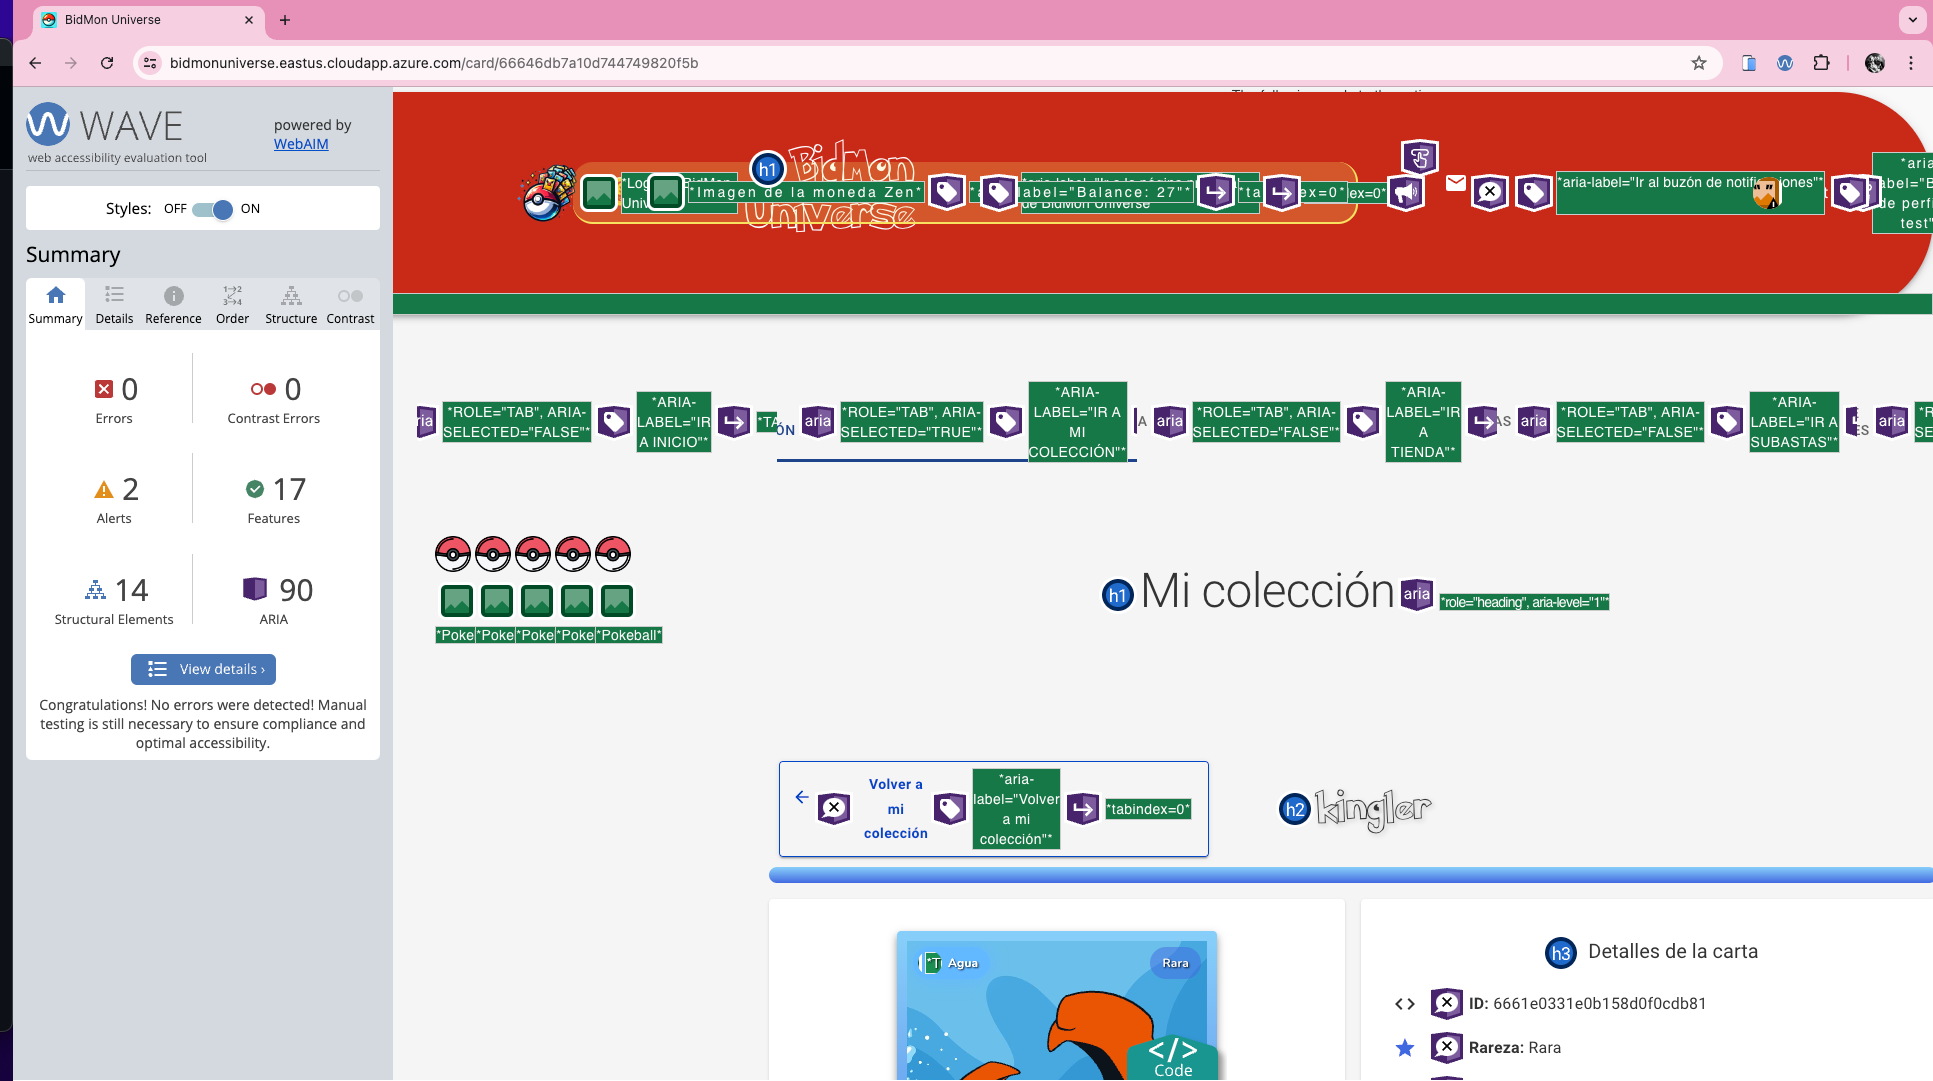
\includegraphics[width=0.8\textwidth]{figures/accesibilidad/A-acc-detalle-carta.png}
    \caption{Accesibilidad Página Detalle de una carta}
    \label{fig:Acc-Detalle-Carta}
\end{figure}


\subsection*{Pujas activas}
\begin{itemize}
    \item \textbf{Resultado:} La vista de pujas activas cumple con los requisitos de accesibilidad.
    \item \textbf{Observaciones:} Si hay pujas activas, se pueden obtener errores de contraste que se deben a los colores de las cartas y son aceptados.
\end{itemize}


\begin{figure}[H]
    \centering
    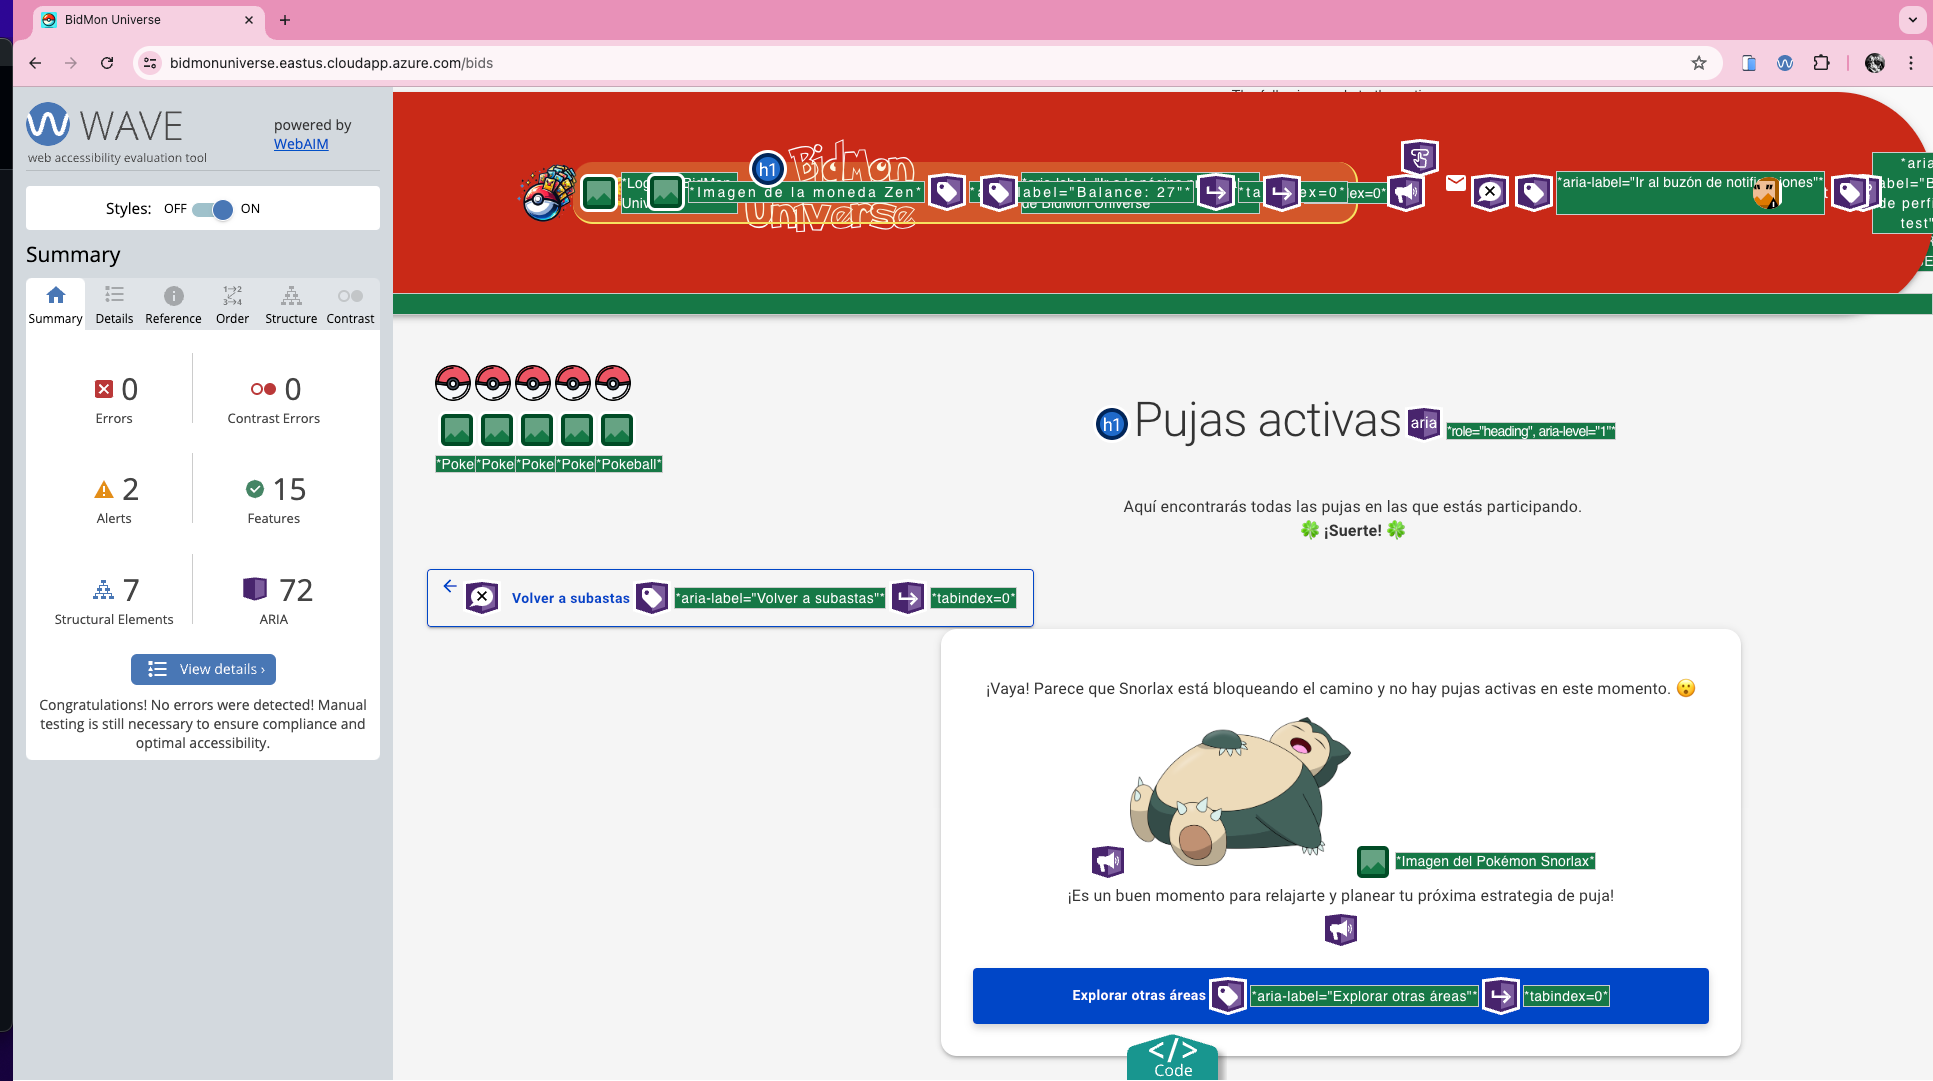
\includegraphics[width=0.8\textwidth]{figures/accesibilidad/A-acc-pujas.png}
    \caption{Accesibilidad Página Pujas activas}
    \label{fig:Acc-Pujas}

\end{figure}


\subsection*{Historial de transacciones}
\begin{itemize}
    \item \textbf{Resultado:} La vista de historial de transacciones cumple con los requisitos de accesibilidad salvo 
    por un error en una etiqueta de formulario.
    \item \textbf{Observaciones:} El error en la etiqueta de formulario se debe a que no se ha asociado correctamente con el campo de entrada,
    en concreto, es en el campo de paginación que crea automáticamente la librería de componentes utilizada.
    Este error no afecta a la accesibilidad de la página, ya que es en la etiqueta de la páginación y no en los propios controles de la tabla.
    Se puede ver detallado en la 
    \coloredUnderline{\hyperlink{fig:Acc-Transacciones-errror}{Figura \ref*{fig:Acc-Transacciones-errror}: \nameref*{fig:Acc-Transacciones-errror}}}.
\end{itemize}

\begin{figure}[H]
    \centering
    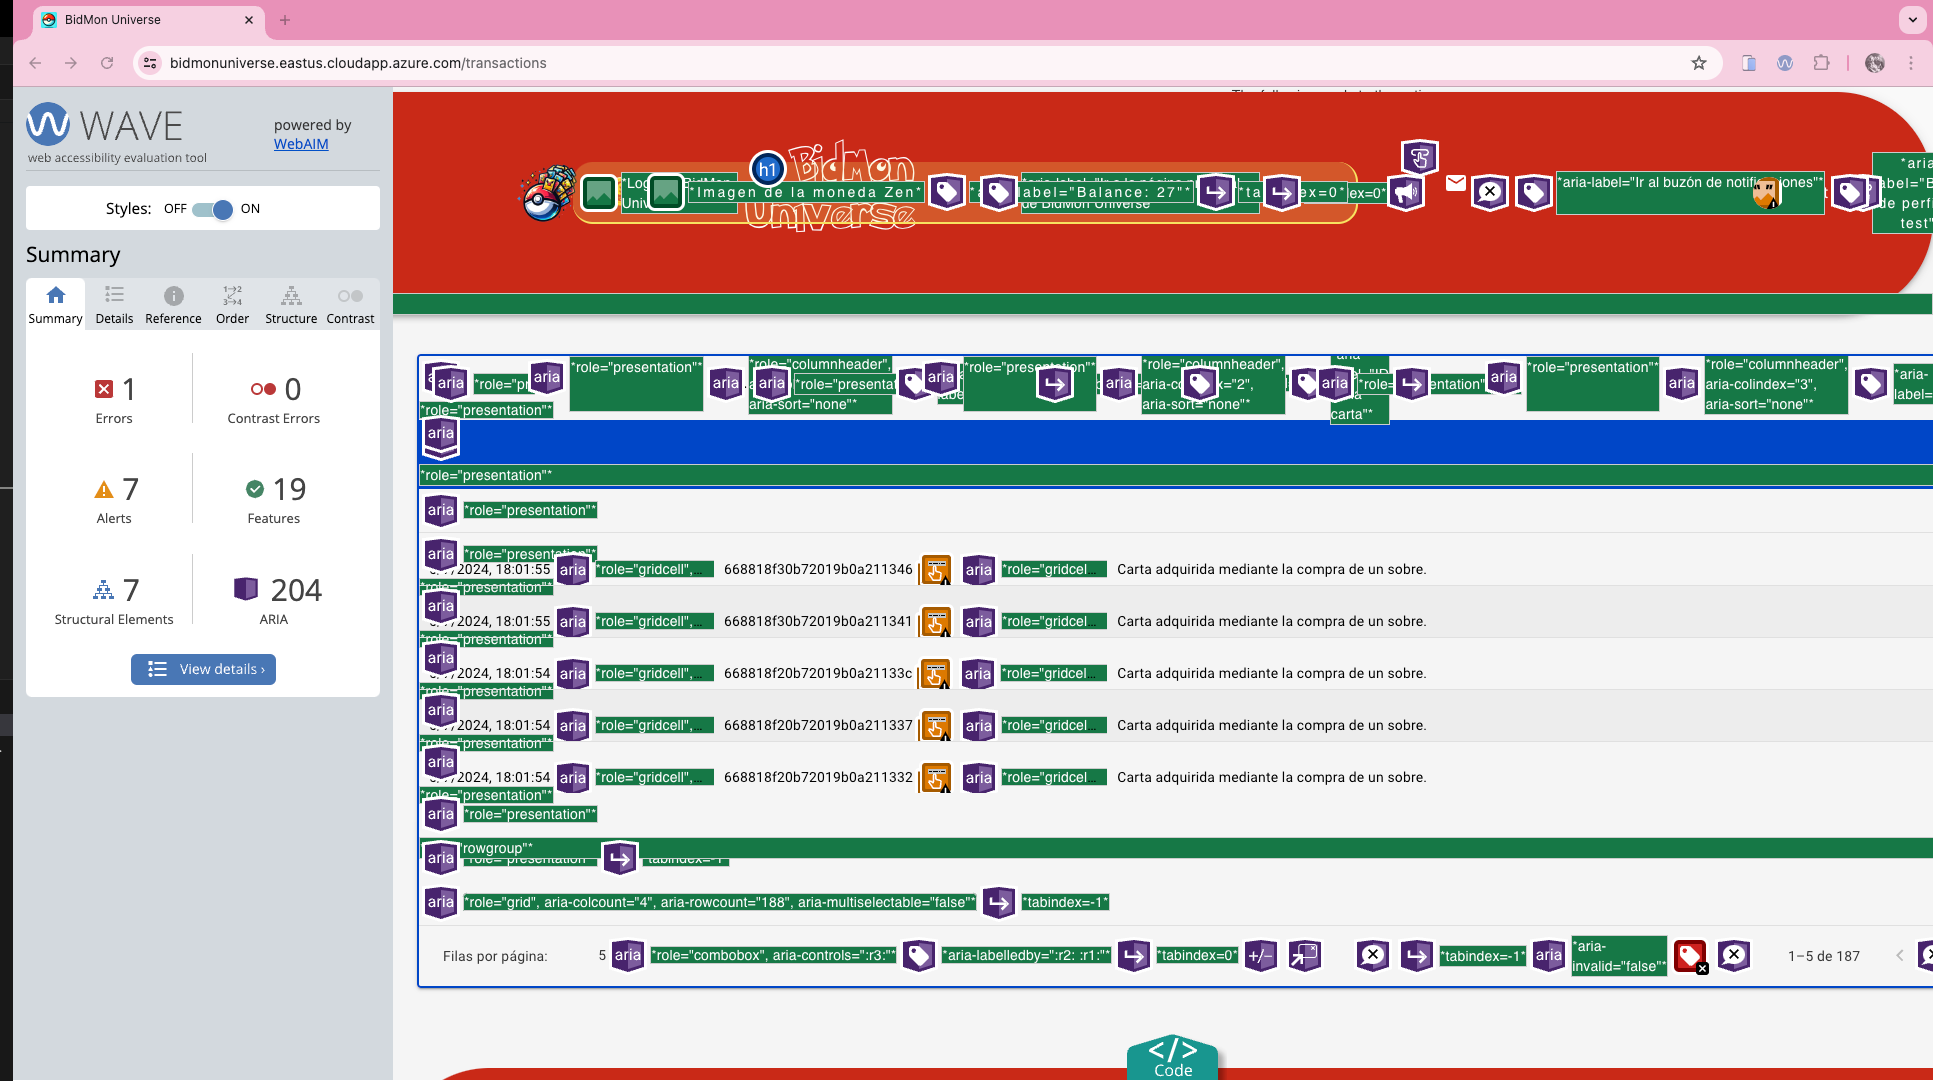
\includegraphics[width=0.8\textwidth]{figures/accesibilidad/A-acc-transacciones.png}
    \caption{Accesibilidad Página Historial de transacciones}
    \label{fig:Acc-Transacciones}
\end{figure}

\begin{figure}[H]
    \centering
    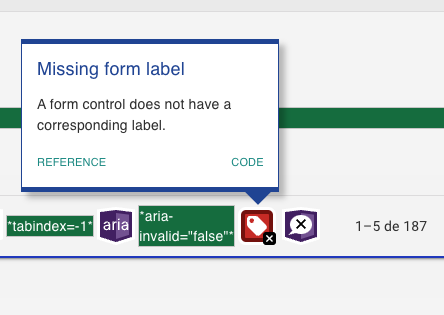
\includegraphics[width=0.8\textwidth]{figures/accesibilidad/A-acc-error-transacciones.png}
    \caption{Accesibilidad Página Historial de transacciones - Error en etiqueta de formulario}
    \label{fig:Acc-Transacciones-errror}
\end{figure}


\subsubsection*{Resumen de resultados}
En general, la aplicación cumple con los requisitos de accesibilidad establecidos en la sección \hyperlink{sec:6_2-RNF}{\ref*{sec:6_2-RNF} \nameref*{sec:6_2-RNF}}.
Se han detectado algunos errores de contraste en las cartas, pero estos son aceptados ya que se deben a los colores 
establecidos en el diseño y no afectan a la accesibilidad de la aplicación.